%
% teil3.tex -- Beispiel-File für Teil 3
%
% (c) 2020 Prof Dr Andreas Müller, Hochschule Rapperswil
%
% !TEX root = ../../buch.tex
% !TEX encoding = UTF-8
%
\section{Anwendungen%
\label{mongekant:section:teil3}}
\kopfrechts{Anwendungen}

Der optimale Transport liefert ein universelles Werkzeug,
um strukturelle Unterschiede zwischen Wahrscheinlichkeitsverteilungen zu quantifizieren.
Nachdem wir in den vorangegangenen Abschnitten
die Grundlagen des optimalen Transports präsentiert haben,
zeigen wir nun,
wie diese Theorie in verschiedenen praktischen Kontexten eingesetzt wird.

Da die Theorie des optimalen Transports auf den ersten Blick abstrakt erscheinen kann,
fokussieren wir uns auf visuelle Anwendungen.
Wir werden die folgenden drei Anwendungen diskutieren:
\begin{enumerate}
\item \emph{Wasserstein-Metrik:}
Wir definieren die wichtigsten Abstände zwischen Verteilungen und
diskutieren ihre mathematischen Eigenschaften
(Abschnitt~\ref{mongekant:subsection:wasserstein}).
\item \emph{Interpolation zwischen Verteilungen:}
Mittels baryzentrischer Mittel interpolieren
wir zwischen ein- und zweidimensionalen Wahrscheinlichkeitsverteilungen
(Abschnitt~\ref{mongekant:subsection:interpolation}).
\item \emph{Farbadaption in der Bildverarbeitung}
Wir zeigen,
wie optimaler Transport zur Angleichung von Farbpaletten
zwischen zwei Bildern genutzt werden kann
(Abschnitt~\ref{mongekant:subsection:farbadaption}).
\end{enumerate}

\subsection{Wasserstein-Metrik%
\label{mongekant:subsection:wasserstein}}

Die Wasserstein-Metrik (auch Kantorowitch-Rubinstein-Metrik genannt)
ist ein Mass für den Abstand zwischen zwei Wahrscheinlichkeitsverteilungen.
Anstatt,
wie z.B. im euklidischen Fall,
punktweise Differenzen zu betrachten,
wird hier die benötigte \glqq Arbeit\grqq gemessen,
um eine Verteilung in die andere zu transformieren.
Da wir genau diese Arbeit im Kantorowitch-Problem minimieren,
erhalten wir als Nebenprodukt die Wasserstein-Metrik.
Diese Idee wird in Abbildung~\ref{mongekant:fig:wasserstein} illustriert.

\begin{figure}
\centering
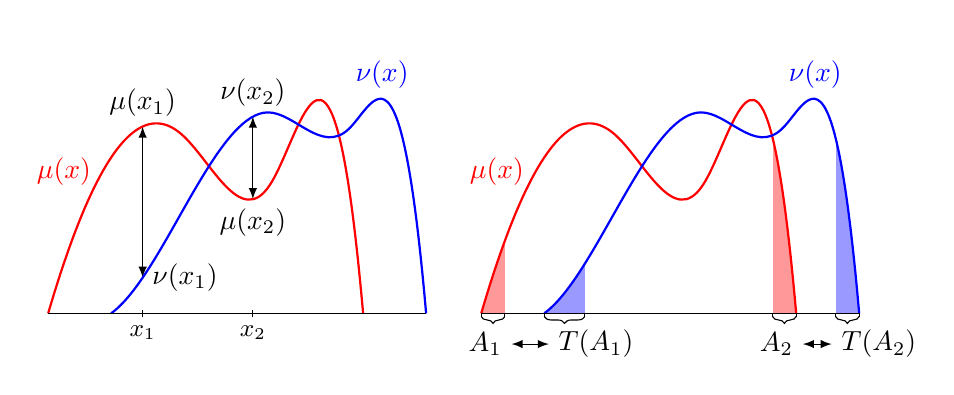
\begin{tikzpicture}[>=latex]
  % Define some colors for consistency
  \def\intensity{0.6}
  \definecolor{lightblue}{rgb}{\intensity, \intensity, 1}
  \definecolor{lightred}{rgb}{1, \intensity, \intensity}
  \def\pathA{(0.000, 0.000) .. controls (0.173, 0.590) and (0.345, 0.976) .. (0.518, 1.131)
   .. controls (0.625, 1.226) and (0.732, 1.233) .. (0.840, 1.143)
   .. controls (1.029, 0.985) and (1.218, 0.528) .. (1.407, 0.814)
   .. controls (1.565, 1.052) and (1.722, 1.807) .. (1.880, 0.975)
   .. controls (1.920, 0.764) and (1.960, 0.450) .. (2.000, 0.000)}
  \def\pathB{(0.000, 0.000) .. controls (0.191, 0.138) and (0.382, 0.541) .. (0.573, 0.857)
   .. controls (0.713, 1.088) and (0.852, 1.272) .. (0.991, 1.276)
   .. controls (1.163, 1.281) and (1.335, 1.008) .. (1.507, 1.169)
   .. controls (1.609, 1.264) and (1.711, 1.512) .. (1.813, 1.238)
   .. controls (1.875, 1.071) and (1.938, 0.709) .. (2.000, 0.000)}
  \def\tickheight{0.02}
  \def\drawscale{2.0}
  \def\xlast{2cm}
  \def\xa{0.6}
  \def\xb{1.3}
  \def\aa{0.15}
  \def\ba{0.258}
  \def\ab{1.85}
  \def\bb{1.850}
  \def\boffset{2.75cm}
  \def\inneroffset{0.4cm}
  \def\arrowoffset{0.8cm}
  \def\bracketoffset{0.35cm}

  % Left Blob (Initial Distribution)
  \begin{scope}[scale=\drawscale,red]
    \draw[<->,black] (\xa, 1.186) node[above]{$\mu(x_1)$} -- (\xa, 0.226) node[right]{$\nu(x_1)$};
    \draw[<->,black] (\xb, 0.725) node[below]{$\mu(x_2)$} -- (\xb, 1.249) node[above]{$\nu(x_2)$};
    \draw[thick] \pathA;
    \node at (0.1cm, 0.9cm) {$\mu(x)$};
    % Right Blob (Transformed Distribution)
    \begin{scope}[xshift=\inneroffset,anchor=south west,color=blue]
      \draw[thick] \pathB node[pos=-0.5,above]{$\nu(x)$};
    \end{scope}

    % Draw Axes
    \begin{scope}[font=\small]
    \draw[black] (0,0) -- (\xlast+\inneroffset,0);
    \draw[black] (\xa,-\tickheight) -- (\xa,\tickheight)
      node[pos=0,anchor=north]{$x_1$} ;
    \draw[black] (\xb,-\tickheight) -- (\xb,\tickheight)
      node[pos=0,anchor=north]{$x_2$} ;
    \end{scope}
  \end{scope}

  % Left Blob (Initial Distribution)
  \begin{scope}[scale=\drawscale,xshift=\boffset,red]
    \begin{scope}[lightred]
      \clip \pathA;
      \fill (0, 0.0) rectangle (\aa, 1.5);
      \fill (\ab, 0.0) rectangle (\xlast, 1.5);
    \end{scope}
    \draw[thick] \pathA;
    \node at (0.1cm, 0.9cm) {$\mu(x)$};
    % Right Blob (Transformed Distribution)
    \begin{scope}[xshift=\inneroffset,anchor=south west,color=blue]
      \begin{scope}[lightblue]
        \clip \pathB;
        \fill (0, 0.0) rectangle (\ba, 1.5);
        \fill (\bb, 0.0) rectangle (\xlast, 1.5);
      \end{scope}
      \draw[thick] \pathB node[pos=-0.5,above]{$\nu(x)$};

      \begin{scope}[black]
        \draw (0,0) -- ++(0, -\tickheight) coordinate (b1tickstart);
        \draw (\ba,0) -- ++(0, -\tickheight) coordinate (b1tickend);
        \draw (\bb,0) -- ++(0, -\tickheight) coordinate (b2tickstart);
        \draw (\xlast,0) -- ++(0, -\tickheight) coordinate (b2tickend);
        \draw[decorate,decoration={brace,mirror}] (b1tickstart) -- (b1tickend)
          node[midway,below=\bracketoffset,anchor=center,xshift=0.4cm](b1end) {$T(A_1)$};
        \draw[decorate,decoration={brace,mirror}] (b2tickstart) -- (b2tickend)
          node[midway,below=\bracketoffset,anchor=center,xshift=0.4cm](b2end) {$T(A_2)$};
      \end{scope}
    \end{scope}
    \begin{scope}[black]
      \draw (0,0) -- (\xlast+\inneroffset,0);

      \draw (0,0) -- ++(0, -\tickheight) coordinate (a1tickstart);
      \draw (\aa,0) -- ++(0, -\tickheight) coordinate (a1tickend);
      \draw (\ab,0) -- ++(0, -\tickheight) coordinate (a2tickstart);
      \draw (\xlast,0) -- ++(0, -\tickheight) coordinate (a2tickend);
      \draw[decorate,decoration={brace,mirror}] (a1tickstart) -- (a1tickend)
        node[midway,below=\bracketoffset,anchor=center,xshift=-0.1cm](a1end){$A_1$};
      \draw[decorate,decoration={brace,mirror}] (a2tickstart) -- (a2tickend)
        node[midway,below=\bracketoffset,anchor=center,xshift=-0.1cm](a2end) {$A_2$};
      \draw[<->] (a1end) -- (b1end);
      \draw[<->] (a2end) -- (b2end);
    \end{scope}
  \end{scope}


\end{tikzpicture}

\caption{Punktweise euklidische Distanz im Vergleich zu Wasserstein-Metrik.}
\label{mongekant:fig:wasserstein}
\end{figure}

Seien $\mu, \nu \in \mathcal{P}(\Omega)$ Wahrscheinlichkeitsmasse
auf einem metrischen Raum $(\Omega, d)$ und $p \in [1, \infty)$.
Dann ist die $p$-Wasserstein-Metrik
\begin{align}
\wasserstein(\mu, \nu)
&:=
\inf_{\gamma \in \Gamma(\mu, \nu)}
\left(
\int_{\Omega \times \Omega} d(x,y)^p\, d\gamma(x,y)
\right)^{1/p}
.
\label{mongekant:eq:wasserstein_metric}
\end{align}
Wenn $p=1$,
dann wird $\wasserstein[1]$ auch häufig Earth-Mover-Distance genannt,
wobei der Namen vom ursprünglichen Problem mit Sandhaufen herrührt.
Die Wasserstein-Metrik ist tatsächlich eine Metrik,
d.h. sie erfüllt die vier Axiome:
\begin{itemize}
\item $\wasserstein(\mu, \mu) = 0$ (Identität)
\item $\wasserstein(\mu, \nu) > 0,$ wobei $\mu \neq \nu$ (Positivität)
\item $\wasserstein(\mu, \nu) = \wasserstein(\nu, \mu)$ (Symmetrie)
\item $\wasserstein(\mu, \rho) \leq \wasserstein(\mu, \nu) + \wasserstein(\nu, \rho)$
(Dreiecksungleichung)
\end{itemize}
Die Beweise für diese Eigenschaften sind allerdings
ausserhalb des Umfangs dieses Seminars.
Wer sich dafür interessiert,
sei auf \cite{mongekant:villani} verwiesen.

\subsection{Baryzentren und Interpolation
\label{mongekant:subsection:interpolation}}

In vielen Anwendungen
(z,B. Bild- und Signalverarbeitung, Statistik, maschinelles Lernen) ist es nötig,
zwei Wahrscheinlichkeitsverteilungen zu \emph{mischen}
oder zu \emph{interpolieren}.
Die naheliegende Idee ist die euklidische Interpolation
\begin{align}
\rho_E(\alpha)
&=
(1-\alpha) \mu + \alpha \nu
\label{mongekant:eq:euclidean_barycenter}
,
\end{align}
wobei $\alpha \in [0,1]$ der Mischparameter ist und $\rho$ die Interpolation.
Falls $\alpha=0$,
dann ist $\rho=\mu$,
während für $\alpha=1$ gilt $\rho=\nu$.
Diese Interpolation ist allerdings nur sinnvoll,
wenn $\mu$ und $\nu$ sehr ähnlich sind und an der selben geometrischen Lage liegen.
Optimaler Transport bietet eine elegante Alternative,
Die Idee ist,
anstatt die Verteilungen direkt zu mischen,
die gewichteten \emph{Baryzentren} der Verteilungen zu berechnen.
Seien $\mu, \nu \in \mathcal{P}(\Omega)$ Wahrscheinlichkeitsmasse
auf einem metrischen Raum $(\Omega, d)$
und $p \in [1, \infty)$.
Dann ist das Wasserstein-Baryzentrum
\begin{align}
\rho_W(\alpha)
&:=
\underset{\rho \in \mathcal{P}(\Omega)}{\mathrm{arg\,min}}\left(
(1-\alpha) \wasserstein(\mu, \rho)
+ \alpha \wasserstein(\nu, \rho)
\right)
\label{mongekant:eq:wasserstein_barycenter}
.
\end{align}
Die Idee ist,
dass das Baryzentrum $\rho(\alpha)$
so gewählt wird,
dass die gewichtete Summe der Abstände zu $\mu$ und $\nu$ minimiert wird.

Die Interpolation mittels Baryzentren
ist in Abbildung~\ref{mongekant:fig:barycenter1d} für 1-dimensionale Verteilungen
und in Abbildung~\ref{mongekant:fig:barycenter2d} für 2-dimensionale Verteilungen
dargestellt.
Es ist klar ersichtlich,
dass die euklidische Interpolation
zu unnatürlichen Mischungen führt,
während die Wasserstein-Interpolation
intuitive Resultate liefert.
Dabei sollte man allerdings beachten,
dass die Berechnung der Wasserstein-Interpolation
deutlich aufwändiger ist als die euklidische Interpolation.

\begin{figure}
\centering
\subfigure[Euklidische Interpolation\label{mongekant:fig:barycenter_ray_euclidean}]{
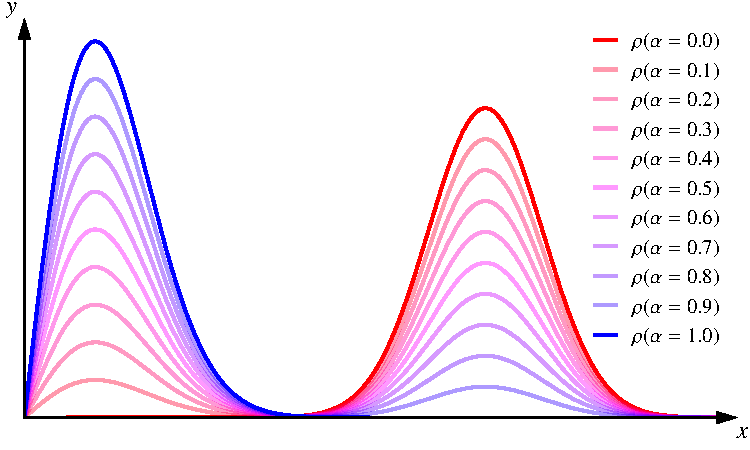
\includegraphics[scale=0.8]{papers/mongekant/code/barycenter_ray_euclidean}
}
\subfigure[Wasserstein-Interpolation mit $d(x,y) = |x - y|^2$.%
\label{mongekant:fig:barycenter_ray_wasserstein}]{
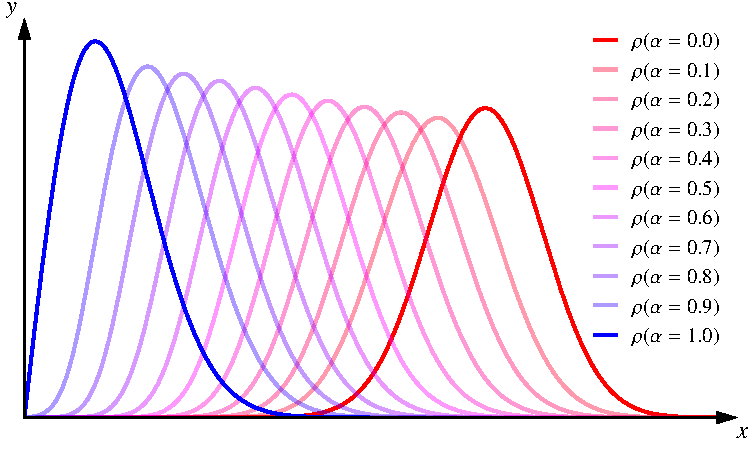
\includegraphics[scale=0.8]{papers/mongekant/code/barycenter_ray_wasserstein}
}
\caption{Interpolation zwischen einer {\color{red}Normal-} und
einer {\color{blue}Rayleigh-}Verteilung}
\label{mongekant:fig:barycenter1d}
\end{figure}


\begin{figure}
\centering
\subfigure[Euklidische Interpolation\label{mongekant:fig:euclidean2d}]{
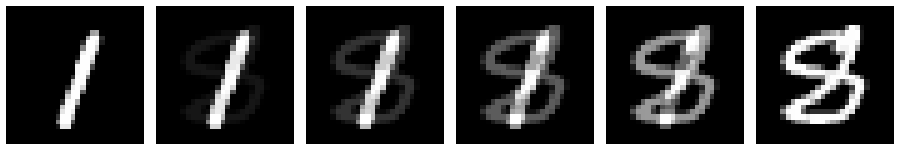
\includegraphics[scale=0.8]{papers/mongekant/code/euclidean2d}
}
\subfigure[Wasserstein-Interpolation mit $d(x,y) = |x - y|^2$.%
\label{mongekant:fig:wasserstein2d}]{
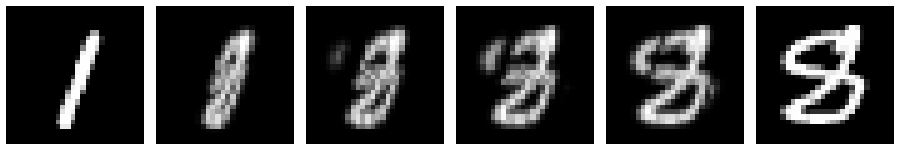
\includegraphics[scale=0.8]{papers/mongekant/code/wasserstein2d}
}
\caption{Interpolation zwischen zwei Bildern}
\label{mongekant:fig:barycenter2d}
\end{figure}


Zudem können wir zeigen,
dass \eqref{mongekant:eq:euclidean_barycenter} das Resultat eines ähnlichen Optimierungsproblems ist,
wobei wir $\wasserstein(\mu, \nu)$ mit $d(\mu, \nu) = (\mu - \nu)^2$ ersetzen:
\begin{align*}
\rho_E(\alpha)
&=
\underset{\rho \in \mathcal{P}(\Omega)}{\mathrm{arg\,min}}\left(
(1-\alpha) (\mu - \rho)^2
+ \alpha (\nu - \rho)^2
\right)
.
\end{align*}
Da es sich hier um ein quadratisches Minimalproblem handelt,
können wir das Problem in die Form
\begin{align*}
f(\rho)
&=
a \rho^2 + b \rho + c
,
\end{align*}
bringen,
um den Scheitelpunkt der Parabel zu finden.
Dann ergibt sich das Minimum an der Stelle
\begin{align}
\rho_E
=
-\frac{b}{2a}
\label{mongekant:eq:qaud}
.
\end{align}
Multiplizieren wir den Ausdruck aus und 
arrangieren die Terme um,
erhalten wir:
\begin{align*}
(1 - \alpha) (\mu - \rho)^2 
+ \alpha (\nu - \rho)^2
&=
(1 - \alpha) \left(\mu^2 - 2\mu\rho + \rho^2 \right)
+ \alpha \left(\nu^2 - 2\nu\rho + \rho^2 \right)
\\
&=
\mu^2 - 2\mu\rho + \rho^2 - \alpha \mu^2 + 2\alpha\mu\rho - \alpha\rho^2 
+ \alpha \nu^2 - 2\alpha\nu\rho + \alpha\rho^2
\\
&=
\underbrace{1}_{\displaystyle a} \rho^2 
+ \underbrace{2 \bigl((\alpha - 1) \mu - \alpha\nu \bigr)}_{\displaystyle b} \rho
+ \underbrace{(1 - \alpha) \mu^2 + \alpha \nu^2}_{\displaystyle c}
.
\end{align*}
Setzen wir die erhaltenen Parameter nun in \eqref{mongekant:eq:qaud} ein,
resultiert
\begin{align*}
\rho_E
&=
-\frac{2 \bigl(\left(\alpha - 1\right) \mu - \alpha\nu \bigr)}{2 \cdot 1}
\\
&=
(1 - \alpha) \mu + \alpha \nu
,
\end{align*}
was exakt \eqref{mongekant:eq:euclidean_barycenter} entspricht.

\subsection{Farbadaption\label{mongekant:subsection:farbadaption}}

Die Farbadaptierung ist eine Technik in der Bildverarbeitung,
bei der die Farbverteilung eines Quellbildes an die eines Zielbildes angepasst wird.
Ziel ist es,
dass das Quellbild nach der Transformation
die farbliche Atmosphäre des Zielbildes widerspiegelt,
während seine geometrische Struktur (Kanten, Formen, Texturen) erhalten bleibt.
Ein Beispielresultat ist in Abbildung~\ref{mongekant:fig:adaption} dargestellt.

\begin{figure}
\centering
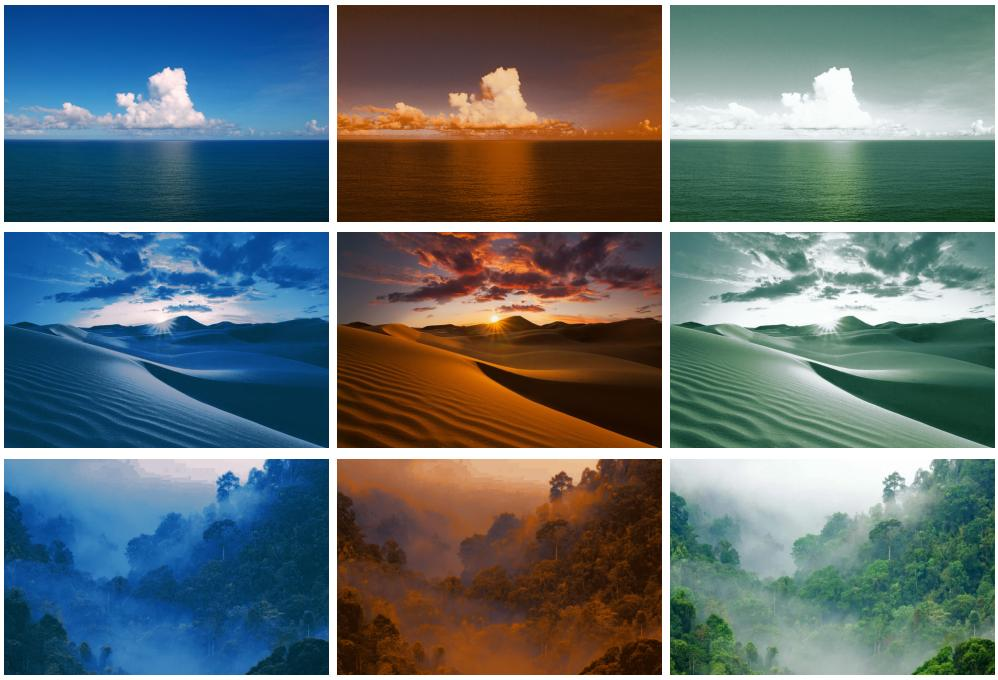
\includegraphics[width=\textwidth]{papers/mongekant/code/adaption}
\caption{Farbadaptierung zwischen Bildern.
Dabei sind die orginalen Bilder in der Diagonalen angeordnet.
Zudem wurde $c(x,y) = |x - y|^2$ als Kostenfunktion verwendet.
}
\label{mongekant:fig:adaption}
\end{figure}

Ein natürlicher Ansatz zur Lösung dieser Aufgabe
basiert auf dem Konzept des optimalen Transports.
Dabei werden die Farbwerte der beiden Bilder
als diskrete Wahrscheinlichkeitsverteilungen im Farbraum (z.\,B. RGB) modelliert.
Man bezeichnet die Farbverteilung des Quellbildes
als Mass $\mu = \sum_{i=1}^n \alpha_i \delta_{x_i}$ und
die des Zielbildes als Mass $\nu = \sum_{j=1}^m \beta_j \delta_{y_j}$,
wobei $x_i, y_j \in \mathbb{R}^d$ Farbwerte und
$\alpha_i, \beta_j$ deren zugehörige Gewichte sind.
Die Kostenfunktion wird typischerweise als $c(x,y) = |x - y|^2$ gewählt.

\subsubsection{Probleme der klassischen Lösung}
In der Praxis weist die Farbverteilung von Bildern
oft Unterschiede in der Dichte und Struktur auf.
So kann z.B. ein Bild grosse einfarbige Flächen enthalten,
während ein anderes viele feine Farbnuancen hat.
Die klassische Methode des optimalen Transports überträgt die Massen strikt 1:1,
was zu unnatürlichen Ergebnissen führen kann:
\begin{itemize}
\item Geringe Farbanteile im Zielbild können
auf grosse Bereiche im Quellbild abgebildet werden.
\item Rauschen im Zielbild wird verstärkt übertragen.
\item Die resultierenden Farben können abrupt wechseln,
ohne Rücksicht auf die lokalen Bildstrukturen.
\end{itemize}

\subsubsection{Relaxierter und regularisierter optimaler Transport}
Um diese Probleme zu vermeiden,
schlägt \cite{mongekant:color} eine \emph{relaxierte und regularisierte}
Variante des optimalen Transports vor.
Dabei wird einerseits die strikte Massenkonservierung gelockert,
andererseits eine Glättung des Transportplans eingeführt.

Die relaxierte Formulierung erlaubt,
dass nicht die gesamte Masse transportiert werden muss.
Dies geschieht durch Einführung von Toleranzen $\tau_\alpha, \tau_\beta > 0$
in den Randbedingungen
\begin{align*}
\left| \sum_{j} \gamma_{ij} - \alpha_i \right|
\leq
\tau_a
, \quad
\left| \sum_{i} \gamma_{ij} - \beta_j \right|
\leq
\tau_b.
\end{align*}
Zusätzlich wird ein Regularisierungsterm $R(\gamma)$ eingeführt,
der räumliche Kohärenz im Transportplan fördert.
Typische Regularisierungen sind:
\begin{align*}
R(\gamma)
&=
\lambda \cdot \mathrm{TV}(\gamma)
\quad \text{oder} \quad
\lambda \cdot |\nabla \gamma|^2,
\end{align*}
wobei $\mathrm{TV}(\gamma)$ die totale Variation \cite{mongekant:totvar}
auf einem Nachbarschaftsgraphen der Quellpunkte beschreibt
und $\nabla$ ein diskreter Gradientoperator ist.
Die resultierende Optimierungsaufgabe lautet
\begin{align*}
\gamma^\ast
&=
\min_{\gamma} \sum_{i,j} c(x_i, y_j)\, \gamma_{ij} + R(\gamma),
\end{align*}
mit $\gamma_{ij} \geq 0$ und relaxierten Randbedingungen.

\subsubsection{Praktische Umsetzung}
Da eine exakte Berechnung auf allen Bildpunkten sehr rechenintensiv wäre,
wird typischerweise eine \emph{Subsampling}-Strategie genutzt.
Hierbei werden Farben beider Bilder auf jeweils $n$ Cluster
(z.B. mittels $k$-Means) reduziert.
Auf diesen Clustern wird das Transportproblem gelöst.
Anschliessend wird das Ergebnis auf die Originalpixel zurückprojiziert,
z.B. mithilfe baryzentrischer Interpolation
\begin{align*}
T(x_i)
=
\frac{1}{\sum_j \gamma^\ast_{ij}} \sum_j \gamma^\ast_{ij} \, y_j.
\end{align*}

